\documentclass[11pt,dvipsnames,usenames,aspectratio=169]{beamer}  % Add handout to options to disable overlays

% For more themes, color themes and font themes, see:
% http://deic.uab.es/~iblanes/beamer_gallery/index_by_theme.html
%
\mode<presentation>
{%
  \usetheme{CambridgeUS}    % or try default, Darmstadt, Warsaw, ...
  \usecolortheme{whale}     % or try albatross, beaver, crane, ...
  \usefonttheme{serif}          % or try default, structurebold, ...
  % \usefonttheme[onlymath]{serif}
  % \setbeamertemplate{navigation symbols}{}
  % \setbeamercovered{transparent}

  \setbeamercolor{title}{fg=white}
  \setbeamerfont{title}{series=\bfseries}
  \setbeamercolor{frametitle}{fg=black}
  \setbeamerfont{frametitle}{series=\bfseries}

  \setbeamercolor{section in head/foot}{fg=white}
  \setbeamerfont{section in head/foot}{series=\bfseries}
  \setbeamercolor{subsection in head/foot}{fg=white}
  \setbeamerfont{subsection in head/foot}{series=\bfseries}
  \setbeamercolor{author in head/foot}{fg=white}
  \setbeamerfont{author in head/foot}{series=\bfseries}
  \setbeamercolor{title in head/foot}{fg=white}
  \setbeamerfont{title in head/foot}{series=\bfseries}

  \setbeamercolor{block title}{use=structure,fg=white,bg=title in head/foot.bg}
  \setbeamerfont{block title}{series=\bfseries}
  \setbeamercolor{block body}{use=structure,fg=black,bg=black!1!white}
}

% Support graying out frame elements
\newcommand{\FrameOpague}{\setbeamercovered{again covered={\opaqueness<1->{40}}}}
% Transition slide
\newcommand{\transitionFrame}[1]{%
{%
  \begin{frame}[plain,noframenumbering]{}{} % the plain option removes the sidebar and header from the title page
    \setbeamertemplate{final page}[text]{\Large \textbf{#1}}
    \usebeamertemplate{final page}
  \end{frame}}
}

% \usepackage{hyperref}     % Loaded automatically by beamer
\usepackage{pgfplots}       % Used to generate embedded plots
\pgfplotsset{compat=1.13}

% Imported via UltiSnips
\usepackage{mathtools} % for "\DeclarePairedDelimiter" macro
\DeclarePairedDelimiter{\floor}{\lfloor}{\rfloor}
\DeclarePairedDelimiter{\ceil}{\lceil}{\rceil}
\DeclarePairedDelimiter{\abs}{\lvert}{\rvert}
\DeclarePairedDelimiter{\norm}{\lVert}{\rVert}
% Imported via UltiSnips
\usepackage{amsmath}
\DeclareMathOperator*{\argmax}{arg\,max}
\DeclareMathOperator*{\argmin}{arg\,min}
\usepackage{amsfonts}  % Used for \mathbb and \mathcal
\usepackage{amssymb}
% Imported via UltiSnips
\usepackage{tikz}
\usetikzlibrary{arrows.meta,decorations.markings,shadows,positioning,calc,backgrounds,shapes,overlay-beamer-styles}
% Packages used for the Convolutional NN drawing
\usepackage{graphicx}
\graphicspath{{./img/}}
\usepackage{color}
\usepackage{pgfplots}
\usepackage{pgf-umlsd}
\usepackage{ifthen}
% Imported via UltiSnips
\usepackage[noend]{algpseudocode}
\usepackage[Algorithm,ruled]{algorithm}
\algnewcommand\algorithmicforeach{\textbf{for each}}
\algdef{S}[FOR]{ForEach}[1]{\algorithmicforeach\ #1\ \algorithmicdo}

\newcommand{\pos}{\mathcal{P}}
\newcommand{\unlabel}{\mathcal{U}}

\usepackage{color}
\newcommand{\blue}[1]{{\color{Blue} #1}}
\newcommand{\red}[1]{{\color{red} #1}}
\newcommand{\green}[1]{{\color{ForestGreen} #1}}

%   Define all symbols that are used throughout the document
\newcommand{\toolname}{DeepPU}
\newcommand{\attLossBase}{ttractive loss}
\newcommand{\attLossCap}{A\attLossBase}
\newcommand{\attLossLow}{a\attLossBase}

\newcommand{\etal}{~et~al.}
\newcommand{\elkan}{Elkan \&~Noto}
\newcommand{\kmnist}{K\=/MNIST}   % Use unbreakable hyphen
\newcommand{\cifarT}{CIFAR\=/10}  % Use unbreakable hyphen

\newcommand{\Pos}{\mathcal{P}}
\newcommand{\Unlabel}{\mathcal{U}}

% Attulsive loss function names
\newcommand{\lAtt}{\mathcal{L}_{\text{Att}}}
\newcommand{\lAttBase}[1]{\mathcal{L}_{\text{Att-}#1}}
\newcommand{\lPosAtt}{\lAttBase{\Pos}}
\newcommand{\lUAtt}{\lAttBase{\Unlabel}}
\newcommand{\lPuBase}[1]{\mathcal{L}_{\text{PU-}#1}}
\newcommand{\lPu}{\lPuBase{\Pos{/}\Unlabel}}
\newcommand{\lPuP}{\lPuBase{\Pos}}
\newcommand{\lPuU}{\lPuBase{\Unlabel}}

\newcommand{\xBase}{\mathbf{x}}
\newcommand{\xDomain}{\mathcal{X}}
\newcommand{\lTrip}{\mathcal{L}_{\text{Triplet}}}
\newcommand{\SiamFunc}{f}
\newcommand{\exA}{\xBase_{a}}
\newcommand{\exP}{\xBase_{p}}
\newcommand{\exN}{\xBase_{n}}

% Symbols used in drawing of Deep PU
\newcommand{\xHatP}{\hat{\xBase}_{p}}
\newcommand{\xHatN}{\hat{\xBase}_{n}}
\newcommand{\zBase}{\mathbf{z}}
\newcommand{\zS}{\zBase_{s}}
\newcommand{\zP}{\zBase_{p}}
\newcommand{\zN}{\zBase_{n}}
% Function names for the DeepPU architecture
\newcommand{\fPU}{g}
\newcommand{\fPUenc}{\fPU_{\text{enc}}}
\newcommand{\fPUp}{\fPU_{p}}
\newcommand{\fPUn}{\fPU_{n}}

% Symbols related to prediction of DeepPU
\newcommand{\distSym}{\delta}
\newcommand{\siamDist}[3]{\puDist{#1\left(#2\right)}{#1\left(#3\right)}}
\newcommand{\puDist}[2]{\distSym\left(#1, #2\right)}
\newcommand{\puDistDiff}{\puDist{\xBase}{\xHatP} - \puDist{\xBase}{\xHatN}}
\newcommand{\sign}[1]{\text{sgn}\Big(#1\Big)}

% Colors
\definecolor{atomictangerine}{rgb}{1.0, 0.6, 0.4}
\definecolor{dartmouthgreen}{rgb}{0.05, 0.5, 0.06}
\definecolor{lust}{rgb}{0.9, 0.13, 0.13}

% Convolutional AE macros
\newcommand{\bfx}{\mathbf{x}}


% Here's where the presentation starts, with the info for the title slide
\title[Deep Positive-Unlabeled Learning]{Positive-Unlabeled Learning using a Deep Hybrid Generative/Discriminative Model}
\author[Zayd Hammoudeh]{%
  \href{mailto:zayd@cs.uoregon.edu}{\textbf{Zayd Hammoudeh}}\inst{1\textsuperscript{*}}  % \textsuperscript{(\Letter)}
  % \and
  % \href{mailto:lowd@cs.uoregon.edu}{Daniel Lowd}\inst{1}
}

\institute[Univ.\ Oregon]{%
  \textsuperscript{1}\textbf{University of Oregon}\\
  Eugene, OR, USA\\
  \texttt{\href{mailto:zayd@cs.uoregon.edu}{zayd@cs.uoregon.edu}}
  % \texttt{{zayd, lowd}@ucsc.edu}
}
\date{\today}


\begin{document}

\begin{frame}
  \titlepage

  % \vspace{20pt}
  \begin{center}
    \textsuperscript{*} Under the supervision of \textbf{Daniel Lowd}
  \end{center}
\end{frame}

\begin{frame}{What is PU Learning?}
  \begin{itemize}[<+->]
    \setlength{\itemsep}{14pt}
    \item PU = Positive-Unlabeled
    \item Form of \blue{\textbf{binary classification}}
    \item Example of \textit{partially-supervised learning}
    \item \green{\textbf{Non-traditional}} training dataset $\mathcal{S} \coloneqq \pos \cup \unlabel$ such that $\pos \cap \unlabel = \emptyset$
      \begin{itemize}[<+->]
        \item $\pos$: Labeled examples all from positive class
        \item $\unlabel$: Unlabeled training set with \blue{\textbf{unknown distribution}} of positive \& negative examples
      \end{itemize}
    \item \textit{Example Applications}: Protein-similarity prediction, land-cover classification, targeted marketing, deceptive/incentivized review identification
      \begin{itemize}[<+->]
        \item Both \blue{inductive} \& \red{transductive} domains
        \item We will focus on the \red{transductive} learning
      \end{itemize}
  \end{itemize}
\end{frame}

\begin{frame}{What is an Autoencoder?}
  \onslide<+->{Neural \textbf{Generative Model}: Reconstructs input (image) from compressed representation}

  \onslide<+->{\vspace{8pt}Used for \textit{Representation Learning} --- typically dimensionality reduction}
  \\\vspace{14pt}
  % Convolutional Autoencoder
% Modified Version Of: https://github.com/jettan/tikz_cnn

\newcommand{\CaeImgHeight}{25mm}%
% Source: https://tex.stackexchange.com/questions/295100/partial-or-entire-image-blurring-in-tikz
%Parameters:
%- at position
%- blur parameter
%- image name
\newcommand\blurredimage[3]{%
  \node[opacity=1.0] (output image) at (#1) {\includegraphics[height=\CaeImgHeight]{#3}};
  \node[opacity=0.2] at (#1+ #2, #2) {\includegraphics[height=\CaeImgHeight]{#3}};
  \node[opacity=0.2] at (#1+-#2, #2) {\includegraphics[height=\CaeImgHeight]{#3}};
  \node[opacity=0.2] at (#1+-#2,-#2) {\includegraphics[height=\CaeImgHeight]{#3}};
  \node[opacity=0.2] at (#1+ #2,-#2) {\includegraphics[height=\CaeImgHeight]{#3}};
}%


\centering
\hspace{9in}\resizebox{\textwidth}{!}{%
  \begin{tikzpicture}%
    \draw[use as bounding box, transparent] (-1.8,-1.8) rectangle (17.2, 3.2);
    % Define the macro.
    % 1st argument: Height and width of the layer rectangle slice.
    % 2nd argument: Depth of the layer slice
    % 3rd argument: X Offset --> use it to offset layers from previously drawn layers.
    % 4th argument: Options for filldraw.
    % 5th argument: Text to be placed below this layer.
    % 6th argument: Y Offset --> Use it when an output needs to be fed to multiple layers that are on the same X offset.
    \newcommand{\networkLayer}[6]{%
      \def\a{#1} % Used to distinguish input resolution for current layer.
      \def\b{0.02} %
      \def\c{#2} % Width of the cube to distinguish number of input channels for current layer.
      \def\t{#3} % X offset for current layer.
      \def\d{#4} % Y offset for current layer.
      % Draw the layer body.
      \draw[line width=0.3mm](\c+\t,0,\d) -- (\c+\t,\a,\d) -- (\t,\a,\d);              % back plane
      \draw[line width=0.3mm](\t,0,\a+\d) -- (\c+\t,0,\a+\d) node[midway,below] {#6} -- (\c+\t,\a,\a+\d) -- (\t,\a,\a+\d) -- (\t,0,\a+\d); % front plane
      \draw[line width=0.3mm](\c+\t,0,\d) -- (\c+\t,0,\a+\d);
      \draw[line width=0.3mm](\c+\t,\a,\d) -- (\c+\t,\a,\a+\d);
      \draw[line width=0.3mm](\t,\a,\d) -- (\t,\a,\a+\d);
      % Recolor visible surfaces
      \filldraw[#5] (\t+\b,\b,\a+\d) -- (\c+\t-\b,\b,\a+\d) -- (\c+\t-\b,\a-\b,\a+\d) -- (\t+\b,\a-\b,\a+\d) -- (\t+\b,\b,\a+\d); % front plane
      \filldraw[#5] (\t+\b,\a,\a-\b+\d) -- (\c+\t-\b,\a,\a-\b+\d) -- (\c+\t-\b,\a,\b+\d) -- (\t+\b,\a,\b+\d);
      % Colored slice.
      \ifthenelse {\equal{#5} {}} %
      {} % Do not draw colored slice if #4 is blank.
      {\filldraw[#5] (\c+\t,\b,\a-\b+\d) -- (\c+\t,\b,\b+\d) -- (\c+\t,\a-\b,\b+\d) -- (\c+\t,\a-\b,\a-\b+\d);} % Else, draw a colored slice.
    } %
    \begin{scope}[shift={(5,0)}]
      \onslide<+->{
        % INPUT
        \node[] (input image) at (-3.75,0.5) {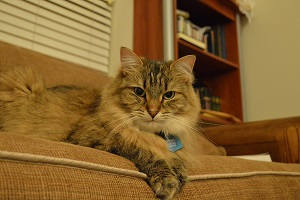
\includegraphics[height=\CaeImgHeight]{tikz/img/muffins.jpg}};
        \node[above of=input image, node distance=1.8cm] {\LARGE $\mathbf{x}$};
        \networkLayer{3.0}{0.03}{-0.5}{0.0}{color=gray!80}{} %
        % ENCODER
        \networkLayer{3.0}{0.1}{0.0}{0.0}{color=white}{}    %
        \networkLayer{2.5}{0.2}{0.4}{0.0}{color=white}{}    %
        \networkLayer{2.0}{0.4}{0.95}{0.0}{color=white}{}   %
        \networkLayer{1.5}{0.4}{1.5}{0.0}{color=white}{}    %
        % BOTTLENECK
        \networkLayer{1.0}{0.4}{2.3}{0.0}{color=red!40}{}    %
        % DECODER
        \networkLayer{1.5}{0.4}{3.3}{0.0}{color=white}{}    %
        \networkLayer{2.0}{0.4}{4.3}{0.0}{color=white}{}    %
        \networkLayer{2.5}{0.2}{5.3}{0.0}{color=white}{}    %
        \networkLayer{3.0}{0.1}{6.2}{0.0}{color=white}{}    %
        % OUTPUT
        \networkLayer{3.0}{0.05}{7.2}{0.0}{color=blue!20}{}  %
        \blurredimage{8.9,0.5}{0.10}{tikz/img/muffins.jpg}  %
        \node[above of=output image, node distance=1.8cm] {\LARGE $\mathbf{\hat{x}}$};
      }
      \onslide<+->{%
        \draw[dashed, blue, thick] (-1.8,3.4) rectangle (2.8,-1.5);
        \node[] () at (-0.3, 3.8) {\blue{\textbf{Encoder}}};
      }
      \onslide<+->{%
        \draw[dashed, color=dartmouthgreen, thick] (1.8,3.4) rectangle (7.5,-1.5);
        \node[] () at (5.4, 3.8) {\textbf{\color{dartmouthgreen} Decoder}};
      }
      \onslide<+->{%
        \draw[color=lust, thick] (1.8,3.4) rectangle (2.8,-1.5);
        \node[] () at (2.3, 3.8) {\textbf{\color{lust} Bottleneck}};
      }
    \end{scope}
  \end{tikzpicture}  %
}

  \\
  \onslide<+->{\centering\Large Objective Function $J = \min \norm{\bfx - \mathbf{\hat{x}}}$}
\end{frame}

\begin{frame}{Basic Idea}
  \begin{itemize}[<+->]
    \setlength{\itemsep}{20pt}
    \item \textbf{Recall}: PU Learning is Binary Classification
      \begin{itemize}[<+->]
        \item \textit{Example}: \blue{\textbf{Positive}}=Cats \& \red{\textbf{Negative}}=Dogs
      \end{itemize}
    \item \textit{Project Intuition}: Simultaneously train two autoencoders (AE):
      \begin{itemize}[<+->]
        \setlength{\itemsep}{6pt}
        \item \textit{Positive AE}: Only reconstruct images of \blue{cats}
        \item \textit{Negative AE}: Only reconstruct images of \red{dogs}
      \end{itemize}

    \item \textbf{Classification}: Assign label matching whichever autoencoder reconstructs input better
  \end{itemize}
\end{frame}

\begin{frame}{Our Architecture}
  \begin{center}
    \scalebox{0.65}{\section{\toolname}\label{sec:Toolname}

Similar to few-shot learning, positive-unlabeled (PU)~learning must overcome limited labeled data.  In fact, PU~learning could be viewed as an instance of zero-shot learning since labeled negative instances are non-existent!  Given this overlap, it may be reasonably expected that ideas originally proposed for Siamese networks may also be applicable to PU~learning.

Shown in Figure~\ref{fig:Toolname}, our deep positive-unlabeled learning architecture, \textit{\toolname}, relies on a bifurcated autoencoder.  Each input ${\xBase\in\xDomain}$ is mapped by encoder~$g_e$ to (concatenated) latent space ${\zBase\in\mathbb{R}^{\abs{\zP}+\abs{\zS}+\abs{\zN}}}$. Unlike Siamese networks which map instances to~$\mathbb{R}^m$, \toolname\ is a function ${\fPU:\xDomain\mapsto\xDomain\times\xDomain}$.  Each instance in the generated tuple corresponds to an output of one of two decoders.  As described in the next section, decoder~$\fPUp$ is trained to accurately reconstruct specifically positive instances while decoder~$\fPUn$ is trained to correctly reconstruct negative instances.

Observe that the positive and negative decoder inputs --- ${\lbrack \zS~\zP \rbrack}$ and ${\lbrack \zS~\zN \rbrack}$ respectively --- are not identical.  The shared latent vector component,~$\zS$, contains the mutual information needed to reconstruct \textit{both} positive and negative instances while $\zP$ and~$\zN$ contain class-specific reconstruction information --- i.e.,~for positive and negative respectively.

\begin{figure}[t]
  \centering
  \section{\toolname}\label{sec:Toolname}

Similar to few-shot learning, positive-unlabeled (PU)~learning must overcome limited labeled data.  In fact, PU~learning could be viewed as an instance of zero-shot learning since labeled negative instances are non-existent!  Given this overlap, it may be reasonably expected that ideas originally proposed for Siamese networks may also be applicable to PU~learning.

Shown in Figure~\ref{fig:Toolname}, our deep positive-unlabeled learning architecture, \textit{\toolname}, relies on a bifurcated autoencoder.  Each input ${\xBase\in\xDomain}$ is mapped by encoder~$g_e$ to (concatenated) latent space ${\zBase\in\mathbb{R}^{\abs{\zP}+\abs{\zS}+\abs{\zN}}}$. Unlike Siamese networks which map instances to~$\mathbb{R}^m$, \toolname\ is a function ${\fPU:\xDomain\mapsto\xDomain\times\xDomain}$.  Each instance in the generated tuple corresponds to an output of one of two decoders.  As described in the next section, decoder~$\fPUp$ is trained to accurately reconstruct specifically positive instances while decoder~$\fPUn$ is trained to correctly reconstruct negative instances.

Observe that the positive and negative decoder inputs --- ${\lbrack \zS~\zP \rbrack}$ and ${\lbrack \zS~\zN \rbrack}$ respectively --- are not identical.  The shared latent vector component,~$\zS$, contains the mutual information needed to reconstruct \textit{both} positive and negative instances while $\zP$ and~$\zN$ contain class-specific reconstruction information --- i.e.,~for positive and negative respectively.

\begin{figure}[t]
  \centering
  \section{\toolname}\label{sec:Toolname}

Similar to few-shot learning, positive-unlabeled (PU)~learning must overcome limited labeled data.  In fact, PU~learning could be viewed as an instance of zero-shot learning since labeled negative instances are non-existent!  Given this overlap, it may be reasonably expected that ideas originally proposed for Siamese networks may also be applicable to PU~learning.

Shown in Figure~\ref{fig:Toolname}, our deep positive-unlabeled learning architecture, \textit{\toolname}, relies on a bifurcated autoencoder.  Each input ${\xBase\in\xDomain}$ is mapped by encoder~$g_e$ to (concatenated) latent space ${\zBase\in\mathbb{R}^{\abs{\zP}+\abs{\zS}+\abs{\zN}}}$. Unlike Siamese networks which map instances to~$\mathbb{R}^m$, \toolname\ is a function ${\fPU:\xDomain\mapsto\xDomain\times\xDomain}$.  Each instance in the generated tuple corresponds to an output of one of two decoders.  As described in the next section, decoder~$\fPUp$ is trained to accurately reconstruct specifically positive instances while decoder~$\fPUn$ is trained to correctly reconstruct negative instances.

Observe that the positive and negative decoder inputs --- ${\lbrack \zS~\zP \rbrack}$ and ${\lbrack \zS~\zN \rbrack}$ respectively --- are not identical.  The shared latent vector component,~$\zS$, contains the mutual information needed to reconstruct \textit{both} positive and negative instances while $\zP$ and~$\zN$ contain class-specific reconstruction information --- i.e.,~for positive and negative respectively.

\begin{figure}[t]
  \centering
  \input{tikz/deep_pu.tex}
  \caption{\toolname\ network architecture}\label{fig:Toolname}
\end{figure}

\subsection{Learning}

This subsection outlines our novel ideas for training \toolname\@.

\paragraph{Loss Function} Just as Siamese network training requires the unique triplet loss, \toolname\ similarly uses a novel loss function we call the \textit{\attLossLow}.

Let $\xBase\in\xDomain$ be a training example with label~${y\in\{\negLabel,\posLabel\}}$. Consider first the more straightforward case where ${\xBase\in\Pos}$ necessitating that ${y=\posLabel}$.  As explained above, \toolname's positive decoder output,~$\xHatP$, should be a more accurate reconstruction of~$\xBase$ than the negative decoder output,~$\xHatN$. If $\xBase$ is considered the ``anchor,'' $\xHatP$ and $\xHatN$ can serve as the triplet loss' $\exP$ and~$\exN$ respectively. The fundamental intuition outlined in Section~\ref{sec:Siamese} still applies.  Our positive \attLossLow\ is shown in Eq.~\eqref{eq:Loss:AttP}.  As with the triplet loss, $\alpha$ is a hyperparameter, and distance metric~$\distSym$'s selection application-specific with mean-squared error often adequate.

\begin{equation}\label{eq:Loss:AttP}
  \lPosAtt = \max\Big\{ \puDistDiff + \alpha, 0 \Big\}
\end{equation}

Consider next the alternative case where ${\xBase\in\Unlabel}$. $y$~is unknown so the triplet loss cannot be directly used, but it helps guide the intuition.

When ${y=\posLabel}$, then during training the distance between~$\xBase$ and~$\exP$ should decrease while the distance between~$\xBase$ and~$\exN$ should increase.  If ${y=\negLabel}$, the direction of changes of these distances is reversed.  $\xBase$~can be thought of as being \textit{attracted} to the decoder associated with its label~$y$. The unlabeled \attLossLow\ in Eq.~\ref{eq:Loss:AttU} modifies the triplet loss to incorporate this attraction.  The basic intuition behind this loss function, put colloquially, is that each ${\xBase\in\Unlabel}$ is driven to ``pick a side'' --- either the positive or negative class.

\begin{equation}\label{eq:Loss:AttU}
  \lUAtt = \max\Big\{ - \big\lvert\puDistDiff\big\rvert + \alpha, 0 \Big\}
\end{equation}

When ${\puDist{\xBase}{\xHatP} < \puDist{\xBase}{\xHatN}}$ --- i.e.,~$\xBase$ appears ``more positive'' --- Eq.~\eqref{eq:Loss:AttU} is equivalent to Eq.~\eqref{eq:Loss:AttP}, and the triplet loss' intuition applies. In the opposite case, where $\xBase$ appears ``more negative'' --- ${\puDist{\xBase}{\xHatN} < \puDist{\xBase}{\xHatP}}$ --- the absolute value inverts the intuition, meaning the loss is minimized when the distance between $\xBase$ and~$\xHatN$ is reduced and the distance between $\xBase$ and~$\xHatP$ increased.

The \attLossLow\ can introduce instability during training since an obvious minimum is to attract all unlabeled instances to one decoder and produce a maximally poor reconstruction on the other decoder.  To ensure minimum reconstruction quality, a reconstruction error term is added to both the positive and unlabeled attractive losses as shown in Eq.~\eqref{eq:Loss:PuP} and Eq.~\eqref{eq:Loss:PuU} respectively. ${\lambda\in\mathbb{R}_{{>}0}}$ is a hyperparameter.

\begin{align}
  \lPuP &= \lPosAtt + \lambda\puDist{\xBase}{\xHatP} \label{eq:Loss:PuP}\\
  \lPuU &= \lUAtt + \underbrace{\lambda\min\Big\{\puDist{\xBase}{\xHatP}, \puDist{\xBase}{\xHatN}\Big\}}_{\text{Reconstruction Quality}}\label{eq:Loss:PuU}
\end{align}

\begin{algorithm}[t]
  \caption{\toolname\ training algorithm}\label{alg:}
  \input{alg/complete_alg.tex}
\end{algorithm}

\paragraph{Training Algorithm} Training is divided into three disjoint phases.  In the first phase, the encoder and negative decoder are fit to minimize the reconstruction error on~$\Unlabel$ similar to a standard, stacked autoencoder; the positive decoder is untouched during this stage.  Once $\Unlabel$'s reconstruction error has adequately converged, training stops, and all weights in the encoder are frozen except those associated exclusively with $\zP$.  This ensures that during the next training phase, the performance of the negative decoder is not degraded.

Stage~2 trains the encoder and positive decoder on~$\Pos$ similar again to a standard autoencoder.  We allow the positive encoder to train for twice as many epochs as the negative decoder.  This increases the likelihood that the positive decoder can reconstruct positive examples more accurately than the negative decoder.  Similarly, since the positive decoder has, until this point, never seen a negative training example, its reconstruction performance on negative instances should be poor.

Before starting the final phase, all networks weights are unfrozen. The encoder and both decoders are then trained on interleaved batches from $\Pos$ and~$\Unlabel$ using the loss functions in Eq.~\eqref{eq:Loss:PuP} and~\eqref{eq:Loss:PuU}.  If hyperparameter $\alpha$ is initially set too high, attraction of unlabeled examples to the positive decoder can be unstable and result in unpredictable network behavior. We address this by setting the initial $\alpha$ close to zero and linearly increasing its value after each epoch.  The previously mentioned batch interleaving also promotes stability be ensuring the performance of both decoders remains in sync.

% \begin{algorithm}[t]
%   \caption{Joint training of the positive and unlabeled decoders}\label{alg:JointTraining}
%   \input{alg/attractive_training.tex}
% \end{algorithm}

\subsection{Inference}

For unlabeled example~${\xBase\in\Unlabel}$, if $g_{p}$ yields a superior reconstruction than $g_{n}$, it can be reasonably concluded that $\xBase$ is positive labeled; otherwise, $\xBase$ is more likely negative labeled.  This intuition is the basis for \toolname's inference function shown in Eq.~\eqref{eq:PU:ClassificationFunc}.

  \begin{equation}\label{eq:PU:ClassificationFunc}
    \hat{y} = -\sign{\puDistDiff}
  \end{equation}

\noindent
In rare cases where ${\puDist{\xBase}{\xHatP}=\puDist{\xBase}{\xHatN}}$, $\xBase$ is equally likely to be either negative or positive labeled.  For simplicity, such examples are assigned a positive label.



  \caption{\toolname\ network architecture}\label{fig:Toolname}
\end{figure}

\subsection{Learning}

This subsection outlines our novel ideas for training \toolname\@.

\paragraph{Loss Function} Just as Siamese network training requires the unique triplet loss, \toolname\ similarly uses a novel loss function we call the \textit{\attLossLow}.

Let $\xBase\in\xDomain$ be a training example with label~${y\in\{\negLabel,\posLabel\}}$. Consider first the more straightforward case where ${\xBase\in\Pos}$ necessitating that ${y=\posLabel}$.  As explained above, \toolname's positive decoder output,~$\xHatP$, should be a more accurate reconstruction of~$\xBase$ than the negative decoder output,~$\xHatN$. If $\xBase$ is considered the ``anchor,'' $\xHatP$ and $\xHatN$ can serve as the triplet loss' $\exP$ and~$\exN$ respectively. The fundamental intuition outlined in Section~\ref{sec:Siamese} still applies.  Our positive \attLossLow\ is shown in Eq.~\eqref{eq:Loss:AttP}.  As with the triplet loss, $\alpha$ is a hyperparameter, and distance metric~$\distSym$'s selection application-specific with mean-squared error often adequate.

\begin{equation}\label{eq:Loss:AttP}
  \lPosAtt = \max\Big\{ \puDistDiff + \alpha, 0 \Big\}
\end{equation}

Consider next the alternative case where ${\xBase\in\Unlabel}$. $y$~is unknown so the triplet loss cannot be directly used, but it helps guide the intuition.

When ${y=\posLabel}$, then during training the distance between~$\xBase$ and~$\exP$ should decrease while the distance between~$\xBase$ and~$\exN$ should increase.  If ${y=\negLabel}$, the direction of changes of these distances is reversed.  $\xBase$~can be thought of as being \textit{attracted} to the decoder associated with its label~$y$. The unlabeled \attLossLow\ in Eq.~\ref{eq:Loss:AttU} modifies the triplet loss to incorporate this attraction.  The basic intuition behind this loss function, put colloquially, is that each ${\xBase\in\Unlabel}$ is driven to ``pick a side'' --- either the positive or negative class.

\begin{equation}\label{eq:Loss:AttU}
  \lUAtt = \max\Big\{ - \big\lvert\puDistDiff\big\rvert + \alpha, 0 \Big\}
\end{equation}

When ${\puDist{\xBase}{\xHatP} < \puDist{\xBase}{\xHatN}}$ --- i.e.,~$\xBase$ appears ``more positive'' --- Eq.~\eqref{eq:Loss:AttU} is equivalent to Eq.~\eqref{eq:Loss:AttP}, and the triplet loss' intuition applies. In the opposite case, where $\xBase$ appears ``more negative'' --- ${\puDist{\xBase}{\xHatN} < \puDist{\xBase}{\xHatP}}$ --- the absolute value inverts the intuition, meaning the loss is minimized when the distance between $\xBase$ and~$\xHatN$ is reduced and the distance between $\xBase$ and~$\xHatP$ increased.

The \attLossLow\ can introduce instability during training since an obvious minimum is to attract all unlabeled instances to one decoder and produce a maximally poor reconstruction on the other decoder.  To ensure minimum reconstruction quality, a reconstruction error term is added to both the positive and unlabeled attractive losses as shown in Eq.~\eqref{eq:Loss:PuP} and Eq.~\eqref{eq:Loss:PuU} respectively. ${\lambda\in\mathbb{R}_{{>}0}}$ is a hyperparameter.

\begin{align}
  \lPuP &= \lPosAtt + \lambda\puDist{\xBase}{\xHatP} \label{eq:Loss:PuP}\\
  \lPuU &= \lUAtt + \underbrace{\lambda\min\Big\{\puDist{\xBase}{\xHatP}, \puDist{\xBase}{\xHatN}\Big\}}_{\text{Reconstruction Quality}}\label{eq:Loss:PuU}
\end{align}

\begin{algorithm}[t]
  \caption{\toolname\ training algorithm}\label{alg:}
  ../../presentation/alg/complete_alg.tex
\end{algorithm}

\paragraph{Training Algorithm} Training is divided into three disjoint phases.  In the first phase, the encoder and negative decoder are fit to minimize the reconstruction error on~$\Unlabel$ similar to a standard, stacked autoencoder; the positive decoder is untouched during this stage.  Once $\Unlabel$'s reconstruction error has adequately converged, training stops, and all weights in the encoder are frozen except those associated exclusively with $\zP$.  This ensures that during the next training phase, the performance of the negative decoder is not degraded.

Stage~2 trains the encoder and positive decoder on~$\Pos$ similar again to a standard autoencoder.  We allow the positive encoder to train for twice as many epochs as the negative decoder.  This increases the likelihood that the positive decoder can reconstruct positive examples more accurately than the negative decoder.  Similarly, since the positive decoder has, until this point, never seen a negative training example, its reconstruction performance on negative instances should be poor.

Before starting the final phase, all networks weights are unfrozen. The encoder and both decoders are then trained on interleaved batches from $\Pos$ and~$\Unlabel$ using the loss functions in Eq.~\eqref{eq:Loss:PuP} and~\eqref{eq:Loss:PuU}.  If hyperparameter $\alpha$ is initially set too high, attraction of unlabeled examples to the positive decoder can be unstable and result in unpredictable network behavior. We address this by setting the initial $\alpha$ close to zero and linearly increasing its value after each epoch.  The previously mentioned batch interleaving also promotes stability be ensuring the performance of both decoders remains in sync.

% \begin{algorithm}[t]
%   \caption{Joint training of the positive and unlabeled decoders}\label{alg:JointTraining}
%   \begin{algorithmic}[1]
  \State Unfreeze all weights
  \State $\alpha \gets 0$
  \While{\text{not converged}}
    \State Increment value of $\alpha$ \Comment{Increasing temperature parameter}
    \While{\text{epoch not complete}}
      \State Select batch $b_{\Pos}$ from $\Pos$
      \State Update $\vec{\theta}$ via $\nabla\lPuP(b_{\Pos})$
      \State Select batch $b_{\Unlabel}$ from $\Unlabel$
      \State Update $\vec{\theta}$ via $\nabla\lPuU(b_{\Unlabel})$
    \EndWhile
  \EndWhile
\end{algorithmic}

% \end{algorithm}

\subsection{Inference}

For unlabeled example~${\xBase\in\Unlabel}$, if $g_{p}$ yields a superior reconstruction than $g_{n}$, it can be reasonably concluded that $\xBase$ is positive labeled; otherwise, $\xBase$ is more likely negative labeled.  This intuition is the basis for \toolname's inference function shown in Eq.~\eqref{eq:PU:ClassificationFunc}.

  \begin{equation}\label{eq:PU:ClassificationFunc}
    \hat{y} = -\sign{\puDistDiff}
  \end{equation}

\noindent
In rare cases where ${\puDist{\xBase}{\xHatP}=\puDist{\xBase}{\xHatN}}$, $\xBase$ is equally likely to be either negative or positive labeled.  For simplicity, such examples are assigned a positive label.



  \caption{\toolname\ network architecture}\label{fig:Toolname}
\end{figure}

\subsection{Learning}

This subsection outlines our novel ideas for training \toolname\@.

\paragraph{Loss Function} Just as Siamese network training requires the unique triplet loss, \toolname\ similarly uses a novel loss function we call the \textit{\attLossLow}.

Let $\xBase\in\xDomain$ be a training example with label~${y\in\{\negLabel,\posLabel\}}$. Consider first the more straightforward case where ${\xBase\in\Pos}$ necessitating that ${y=\posLabel}$.  As explained above, \toolname's positive decoder output,~$\xHatP$, should be a more accurate reconstruction of~$\xBase$ than the negative decoder output,~$\xHatN$. If $\xBase$ is considered the ``anchor,'' $\xHatP$ and $\xHatN$ can serve as the triplet loss' $\exP$ and~$\exN$ respectively. The fundamental intuition outlined in Section~\ref{sec:Siamese} still applies.  Our positive \attLossLow\ is shown in Eq.~\eqref{eq:Loss:AttP}.  As with the triplet loss, $\alpha$ is a hyperparameter, and distance metric~$\distSym$'s selection application-specific with mean-squared error often adequate.

\begin{equation}\label{eq:Loss:AttP}
  \lPosAtt = \max\Big\{ \puDistDiff + \alpha, 0 \Big\}
\end{equation}

Consider next the alternative case where ${\xBase\in\Unlabel}$. $y$~is unknown so the triplet loss cannot be directly used, but it helps guide the intuition.

When ${y=\posLabel}$, then during training the distance between~$\xBase$ and~$\exP$ should decrease while the distance between~$\xBase$ and~$\exN$ should increase.  If ${y=\negLabel}$, the direction of changes of these distances is reversed.  $\xBase$~can be thought of as being \textit{attracted} to the decoder associated with its label~$y$. The unlabeled \attLossLow\ in Eq.~\ref{eq:Loss:AttU} modifies the triplet loss to incorporate this attraction.  The basic intuition behind this loss function, put colloquially, is that each ${\xBase\in\Unlabel}$ is driven to ``pick a side'' --- either the positive or negative class.

\begin{equation}\label{eq:Loss:AttU}
  \lUAtt = \max\Big\{ - \big\lvert\puDistDiff\big\rvert + \alpha, 0 \Big\}
\end{equation}

When ${\puDist{\xBase}{\xHatP} < \puDist{\xBase}{\xHatN}}$ --- i.e.,~$\xBase$ appears ``more positive'' --- Eq.~\eqref{eq:Loss:AttU} is equivalent to Eq.~\eqref{eq:Loss:AttP}, and the triplet loss' intuition applies. In the opposite case, where $\xBase$ appears ``more negative'' --- ${\puDist{\xBase}{\xHatN} < \puDist{\xBase}{\xHatP}}$ --- the absolute value inverts the intuition, meaning the loss is minimized when the distance between $\xBase$ and~$\xHatN$ is reduced and the distance between $\xBase$ and~$\xHatP$ increased.

The \attLossLow\ can introduce instability during training since an obvious minimum is to attract all unlabeled instances to one decoder and produce a maximally poor reconstruction on the other decoder.  To ensure minimum reconstruction quality, a reconstruction error term is added to both the positive and unlabeled attractive losses as shown in Eq.~\eqref{eq:Loss:PuP} and Eq.~\eqref{eq:Loss:PuU} respectively. ${\lambda\in\mathbb{R}_{{>}0}}$ is a hyperparameter.

\begin{align}
  \lPuP &= \lPosAtt + \lambda\puDist{\xBase}{\xHatP} \label{eq:Loss:PuP}\\
  \lPuU &= \lUAtt + \underbrace{\lambda\min\Big\{\puDist{\xBase}{\xHatP}, \puDist{\xBase}{\xHatN}\Big\}}_{\text{Reconstruction Quality}}\label{eq:Loss:PuU}
\end{align}

\begin{algorithm}[t]
  \caption{\toolname\ training algorithm}\label{alg:}
  ../../presentation/alg/complete_alg.tex
\end{algorithm}

\paragraph{Training Algorithm} Training is divided into three disjoint phases.  In the first phase, the encoder and negative decoder are fit to minimize the reconstruction error on~$\Unlabel$ similar to a standard, stacked autoencoder; the positive decoder is untouched during this stage.  Once $\Unlabel$'s reconstruction error has adequately converged, training stops, and all weights in the encoder are frozen except those associated exclusively with $\zP$.  This ensures that during the next training phase, the performance of the negative decoder is not degraded.

Stage~2 trains the encoder and positive decoder on~$\Pos$ similar again to a standard autoencoder.  We allow the positive encoder to train for twice as many epochs as the negative decoder.  This increases the likelihood that the positive decoder can reconstruct positive examples more accurately than the negative decoder.  Similarly, since the positive decoder has, until this point, never seen a negative training example, its reconstruction performance on negative instances should be poor.

Before starting the final phase, all networks weights are unfrozen. The encoder and both decoders are then trained on interleaved batches from $\Pos$ and~$\Unlabel$ using the loss functions in Eq.~\eqref{eq:Loss:PuP} and~\eqref{eq:Loss:PuU}.  If hyperparameter $\alpha$ is initially set too high, attraction of unlabeled examples to the positive decoder can be unstable and result in unpredictable network behavior. We address this by setting the initial $\alpha$ close to zero and linearly increasing its value after each epoch.  The previously mentioned batch interleaving also promotes stability be ensuring the performance of both decoders remains in sync.

% \begin{algorithm}[t]
%   \caption{Joint training of the positive and unlabeled decoders}\label{alg:JointTraining}
%   \begin{algorithmic}[1]
  \State Unfreeze all weights
  \State $\alpha \gets 0$
  \While{\text{not converged}}
    \State Increment value of $\alpha$ \Comment{Increasing temperature parameter}
    \While{\text{epoch not complete}}
      \State Select batch $b_{\Pos}$ from $\Pos$
      \State Update $\vec{\theta}$ via $\nabla\lPuP(b_{\Pos})$
      \State Select batch $b_{\Unlabel}$ from $\Unlabel$
      \State Update $\vec{\theta}$ via $\nabla\lPuU(b_{\Unlabel})$
    \EndWhile
  \EndWhile
\end{algorithmic}

% \end{algorithm}

\subsection{Inference}

For unlabeled example~${\xBase\in\Unlabel}$, if $g_{p}$ yields a superior reconstruction than $g_{n}$, it can be reasonably concluded that $\xBase$ is positive labeled; otherwise, $\xBase$ is more likely negative labeled.  This intuition is the basis for \toolname's inference function shown in Eq.~\eqref{eq:PU:ClassificationFunc}.

  \begin{equation}\label{eq:PU:ClassificationFunc}
    \hat{y} = -\sign{\puDistDiff}
  \end{equation}

\noindent
In rare cases where ${\puDist{\xBase}{\xHatP}=\puDist{\xBase}{\xHatN}}$, $\xBase$ is equally likely to be either negative or positive labeled.  For simplicity, such examples are assigned a positive label.


}
  \end{center}

  \blue{\textbf{Components}}:
  \begin{itemize}
    \setlength{\itemsep}{4pt}
    \onslide<2->{\item Shared input encoder}
    \onslide<3->{\item Latent vector $\mathbf{z}$ partitioned into three parts}
    \onslide<4->{\item $g_{p}$: Decoder for \blue{positive}-examples}
    \onslide<5->{\item $g_{n}$: Decoder for \red{negative}-examples}
  \end{itemize}
\end{frame}

\begin{frame}{Custom Loss Functions}
  ``\blue{\textbf{Attractive}}'' Loss for~$\pos$
  \begin{equation}\label{eq:Loss:AttP}
    \lPosAtt = \max\Big\{ \puDistDiff + \alpha, 0 \Big\}
  \end{equation}

  \vfill
  ``\green{\textbf{Pick-a-Side}}'' Loss for~$\unlabel$
  \begin{equation}\label{eq:Loss:AttU}
    \lUAtt = \max\Big\{ - \big\lvert\puDistDiff\big\rvert + \alpha, 0 \Big\}
  \end{equation}

  \vfill
  Unfortunately, there is no time now to discuss these, but we can in Q\&A if interested\ldots
\end{frame}

\begin{frame}{Training Algorithm (Sketch)}
  ../../presentation/alg/complete_alg.tex
\end{frame}

\begin{frame}{Experiments}
  \begin{itemize}
    \setlength{\itemsep}{16pt}
    \item \blue{\textbf{Dataset}}: MNIST
      \begin{itemize}
        \item \textit{Positive Class}: $4$
        \item \textit{Negative Class}: $9$
      \end{itemize}
    \item \blue{\textbf{Baseline}}: Elkan \& Noto with Logistic Regression
    \item \blue{\textbf{Dataset Sizes}}:
      \begin{itemize}
        \item $\abs{\pos}$: ${\sim}$3,000
        \item $\abs{\unlabel}$: ${\sim}$6,000 evenly split between positive \& negative classes
      \end{itemize}
    \item \blue{\textbf{Labeling Frequency}}: 50\%
  \end{itemize}

  \vspace{16pt}
  Let's look how an example matches our earlier intuition\ldots
\end{frame}

\begin{frame}{Decoder Outputs --- Epoch \red{0}}
  \begin{columns}
    \begin{column}{0.59\textwidth}
      \begin{center}
        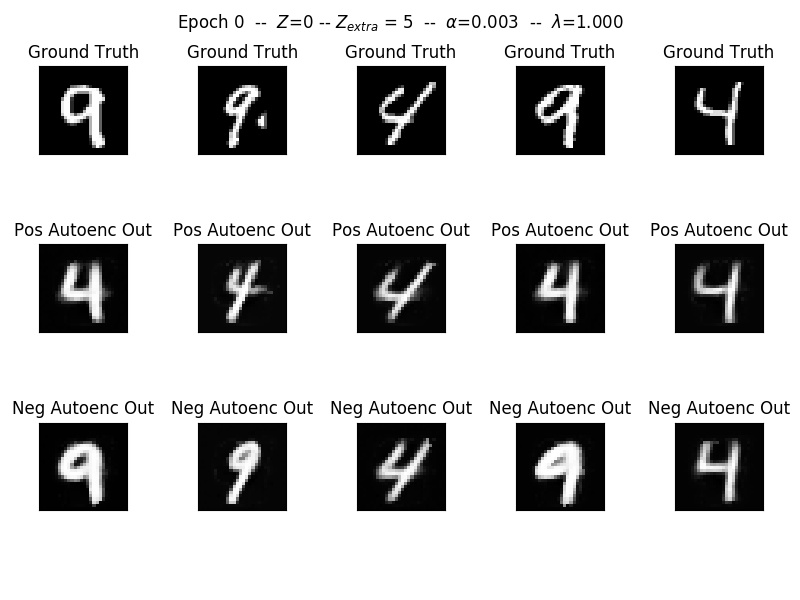
\includegraphics[scale=0.44]{deep-pu_epoch=000.jpg}
      \end{center}
    \end{column}
    \begin{column}{0.41\textwidth}
      \begin{itemize}[<+->]
        \setlength{\itemsep}{20pt}
        \item Positive decoder reconstructs everything as~4
        \item Negative decoder reconstructs both~4 and~9
      \end{itemize}
    \end{column}
  \end{columns}
\end{frame}

\begin{frame}{Decoder Outputs --- Epoch \red{1}}
  \begin{columns}
    \begin{column}{0.59\textwidth}
      \begin{center}
        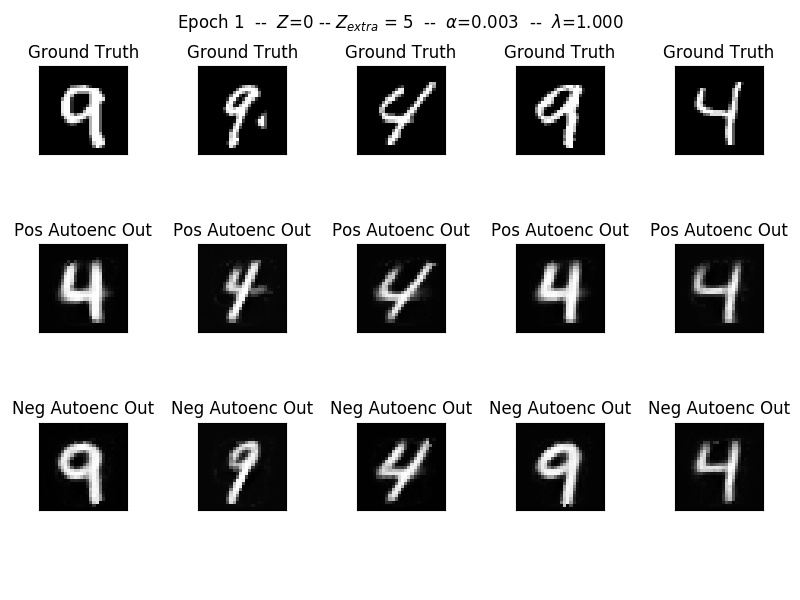
\includegraphics[scale=0.44]{deep-pu_epoch=001.jpg}
      \end{center}
    \end{column}
    \begin{column}{0.41\textwidth}
      \begin{itemize}[<+->]
        \setlength{\itemsep}{20pt}
        \item Not much change after one epoch
      \end{itemize}
    \end{column}
  \end{columns}
\end{frame}

\begin{frame}{Decoder Outputs --- Epoch \red{10}}
  \begin{columns}
    \begin{column}{0.59\textwidth}
      \begin{center}
        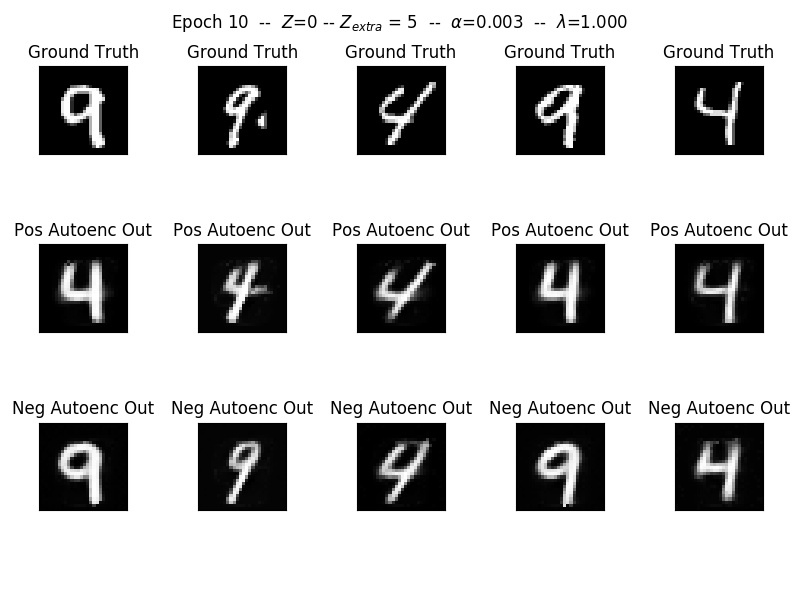
\includegraphics[scale=0.44]{deep-pu_epoch=010.jpg}
      \end{center}
    \end{column}
    \begin{column}{0.41\textwidth}
      \begin{itemize}[<+->]
        \setlength{\itemsep}{20pt}
        \item Positive decoder still unchanged
        \item Negative decoder starting to close \blue{$4$}s to form \red{$9$}s
      \end{itemize}
    \end{column}
  \end{columns}
\end{frame}

\begin{frame}{Decoder Outputs --- Epoch \red{20}}
  \begin{columns}
    \begin{column}{0.59\textwidth}
      \begin{center}
        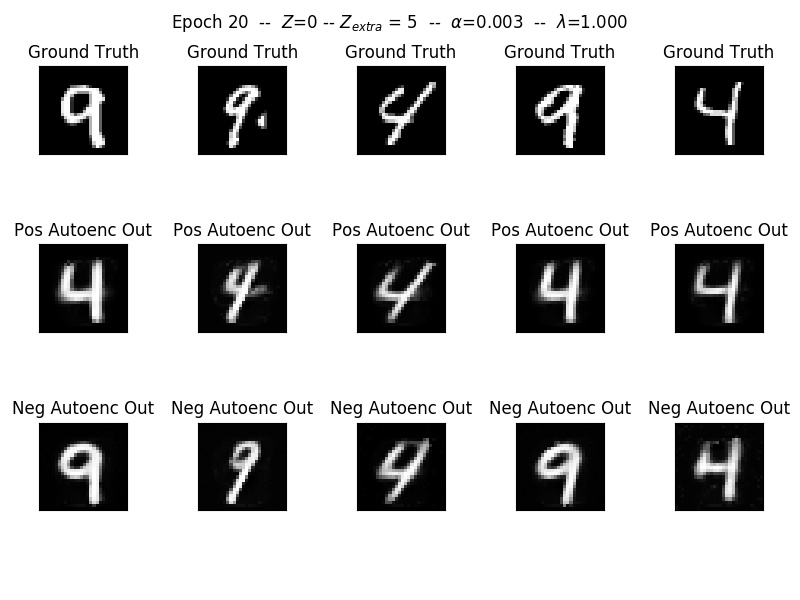
\includegraphics[scale=0.44]{deep-pu_epoch=020.jpg}
      \end{center}
    \end{column}
    \begin{column}{0.41\textwidth}
      \begin{itemize}[<+->]
        \setlength{\itemsep}{20pt}
        \item Positive decoder still unchanged
        \item Negative decoder turning \blue{$4$}s into \red{$9$}s even more
      \end{itemize}
    \end{column}
  \end{columns}
\end{frame}

\begin{frame}{Decoder Outputs --- Epoch \red{50}}
  \begin{columns}
    \begin{column}{0.59\textwidth}
      \begin{center}
        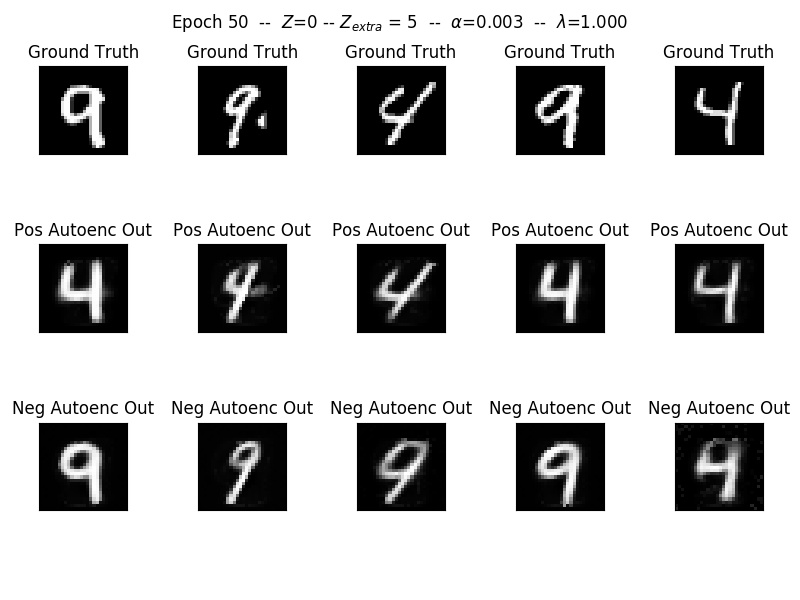
\includegraphics[scale=0.44]{deep-pu_epoch=050.jpg}
      \end{center}
    \end{column}
    \begin{column}{0.41\textwidth}
      \begin{itemize}[<+->]
        \setlength{\itemsep}{20pt}
        \item Positive decoder still unchanged
        \item Negative decoder almost entirely closes input \blue{$4$}s
      \end{itemize}
    \end{column}
  \end{columns}
\end{frame}

\begin{frame}{Decoder Outputs --- Epoch \red{100}}
  \begin{columns}
    \begin{column}{0.59\textwidth}
      \begin{center}
        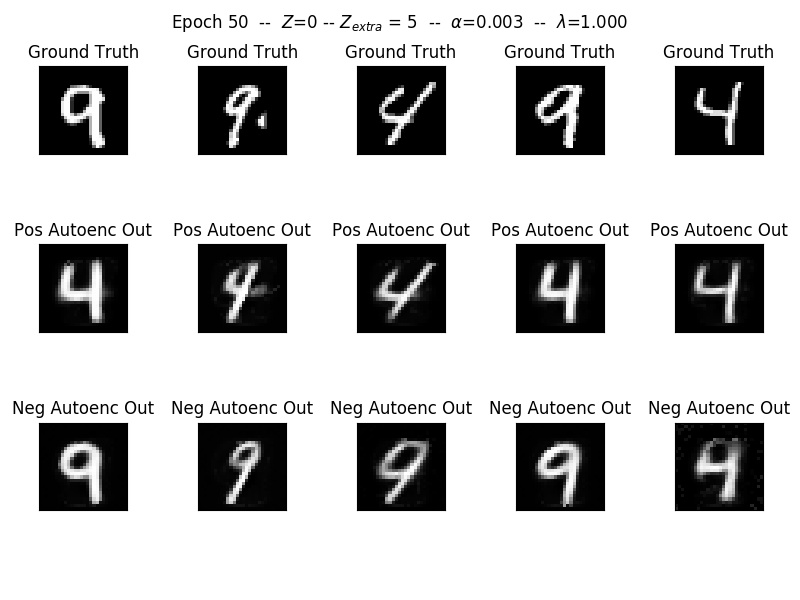
\includegraphics[scale=0.44]{deep-pu_epoch=050.jpg}
      \end{center}
    \end{column}
    \begin{column}{0.41\textwidth}
      \begin{itemize}[<+->]
        \setlength{\itemsep}{20pt}
        \item Positive \& negative decoders always reconstruct \blue{$4$}s \& \red{$9$}s respectively
        \item Suitable to use the generative model as a discriminative classifier
      \end{itemize}
    \end{column}
  \end{columns}
\end{frame}

\begin{frame}{Quantitative Results}
  \begin{itemize}
    \setlength{\itemsep}{15pt}
    \onslide<+->{
      \item \blue{\textbf{Our Architecture}}:
        \begin{itemize}
          \item \textit{Accuracy}: 98.0\%
          \item \textit{AUC ROC}: 0.996
          \item \textit{F1 Score}: 0.980
        \end{itemize}
    }
    \onslide<+->{
      \item \green{\textbf{Elkan \& Noto}}: Using Logistic Regression
        \begin{itemize}
          \item Discussion of this algorithm is beyond the scope of this talk.
          \item \textit{Accuracy}: 89.9\%
          \item \textit{AUC ROC}: 0.969
          \item \textit{F1~Score}: 0.932
        \end{itemize}
    }
  \end{itemize}
\end{frame}

\begin{frame}[allowframebreaks]
  {\tiny
    \frametitle{References}
    \bibliographystyle{ieeetr}
    \bibliography{bib/ref.bib}
  }
\end{frame}

\appendix
\begin{frame}{Previous Work}
  \onslide<+->{\textbf{Two Primary Paradigms}}
  \begin{itemize}[<+->]
    \setlength{\itemsep}{16pt}
    \item ``\blue{\textbf{One Stage Approach}}''
      \begin{itemize}[<+->]
        \setlength{\itemsep}{4pt}
      \item \textit{Heuristically} extract ``reliable negative'' examples~$\mathcal{N}'\in\unlabel$
        \item Train binary classifier $\pos$ vs.\ $\mathcal{N}'$
        \item \red{Disadvantage}: Heuristic-based with high variance based on $\mathcal{N}'$ extraction
      \end{itemize}

    \item ``\blue{\textbf{Two Stage Approach}}''
      \begin{itemize}[<+->]
        \setlength{\itemsep}{4pt}
        \item Cost-sensitive optimization framework
        \item Assume all examples in~$\mathcal{U}$ are negative with a label weight proportional to confidence sample is negative
        \item Train binary classifier $\pos$ vs.\ $\unlabel$
      \end{itemize}
  \end{itemize}

  \vspace{10pt}
  \onslide<+->{\green{\textbf{Baseline for Comparison}}: Seminal two stage approach from Elkan \& Noto~\cite{Elkan:2008}}
\end{frame}

\end{document}
